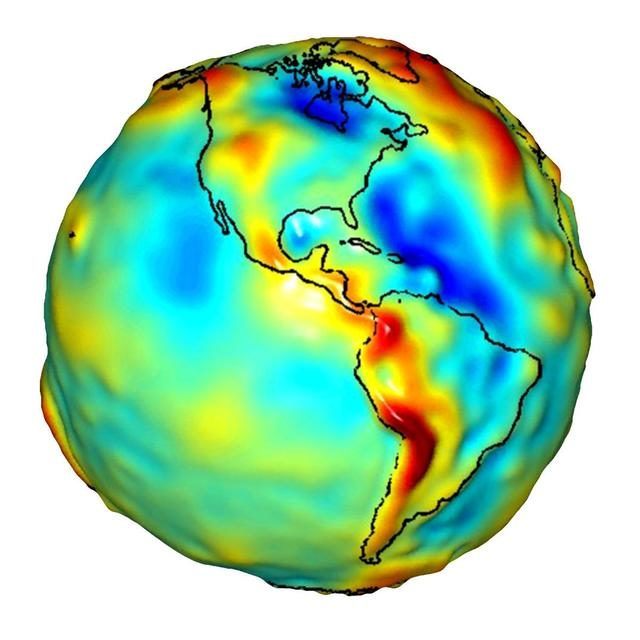
\includegraphics[height=1.25cm]{images/pictograms/gravity}
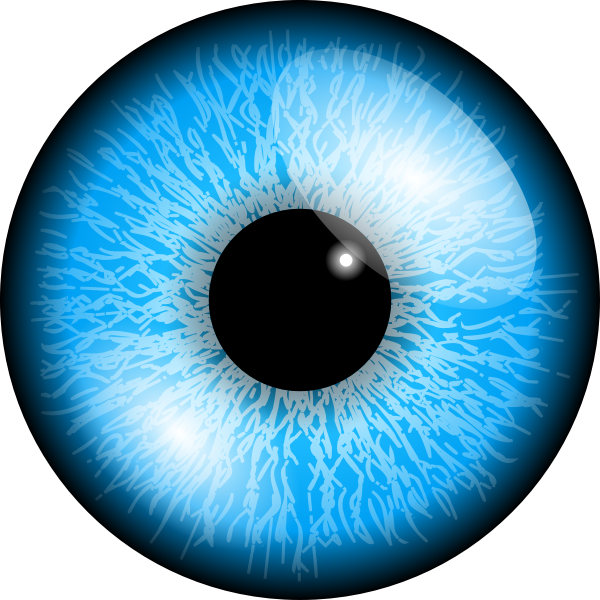
\includegraphics[height=1.25cm]{images/pictograms/visualisation}

\includegraphics[height=1.25cm]{images/pictograms/3d}

%%%%%%%%%%%%%%%%%%%%%%%%%%%%%%%%%%%%%%%%%%%%%%%%%%%%%%%%%%%%%%%%%%%%%%%%%%%%%%%%%%%%%%%%%%%%%%%%%%%

\begin{flushright} {\tiny {\color{gray} python\_codes/fieldstone\_100/text.tex}} \end{flushright}

%\lstinputlisting[language=bash,basicstyle=\small]{python_codes/fieldstone_100/keywords.ascii}

\begin{center}
Code at \url{https://github.com/cedrict/fieldstone/tree/master/python_codes/fieldstone_100}
\end{center}

\par\noindent\rule{\textwidth}{0.4pt}

{\sl This fieldstone was developed in collaboration with B. Root}. \index{contributors}{B. Root}

\par\noindent\rule{\textwidth}{0.4pt}
%%%%%%%%%%%%%%%%%%%%%%%%%%%%%%%%%%%%%%%%%%%%%%%%%%%%%%%%%%%%%%%%%%%%%%%%%%%%%%%%%%%%%%%%%%%%%%

Very high resolution topography datasets of Mars are available at 
\url{https://astrogeology.usgs.gov/search/details/Mars/GlobalSurveyor/MOLA/Mars_MGS_MOLA_DEM_mosaic_global_463m/cub}.
However the data format is not very convenient so Bart Root 
helped me out and exported the data to ascii format.

The file {\filenamefont MOLA\_1deg.txt} counts 64,800 lines, 
i.e. 360x180 points. Longitude values range from  
0.5 to 359.5 and latitudes from -89.5 to +89.5. 

The file {\filenamefont MOLA\_0.5deg.txt} counts 4 times as many lines, 
i.e. 720x360 points=259,200. Longitude values range from  
0.25 to 359.75 and latitudes from -89.75 to +89.75. 

The file {\filenamefont MOLA\_0.25deg.txt} counts 4 times as many lines, 
i.e. 1,036,800 points.

The file {\filenamefont MOLA\_0.0625deg.txt} counts 16 times as many lines, 
i.e. 16,588,800 points.

We follow a similar approach as in \stone 97 and use the data to produce 
two vtu files, one on a 2D plane, one on a 3D sphere:

\begin{center}
\includegraphics[width=15cm]{python_codes/fieldstone_100/images/topo2D_a}\\
\includegraphics[width=5cm]{python_codes/fieldstone_100/images/topo2D_b}
\includegraphics[width=5cm]{python_codes/fieldstone_100/images/topo2D_c}
\includegraphics[width=5cm]{python_codes/fieldstone_100/images/topo2D_d}\\
\includegraphics[width=5cm]{python_codes/fieldstone_100/images/topo3D_1}
\includegraphics[width=5cm]{python_codes/fieldstone_100/images/topo3D_4}
\includegraphics[width=5cm]{python_codes/fieldstone_100/images/topo3D_2}\\
\includegraphics[width=5cm]{python_codes/fieldstone_100/images/topo3D_5}
\includegraphics[width=5cm]{python_codes/fieldstone_100/images/topo3D_3}
\includegraphics[width=5cm]{python_codes/fieldstone_100/images/topo3D_6}\\
{\captionfont Based on the 0.0625degree resolution file.}
\end{center}

Note that the files corresponding to 1/2, 1/4, and 1/16 of degree are not on github since they are quite large. 
Please contact me.

%-------------------------------------------------------------------
\subsection*{Using the topography to compute its gravity signal}

Each cell is characterised by a min/max latitude, longitude. We can convert these to 
spherical coordinates with $\phi$ being the longitude and $\theta$ being the colatitude.
The topography is given with respect to the Mars radius $R_{mars}$. Since the minimum 
of the topography is about $-8.177~\si{\km}$ we define the inner radius of the hollow planet 
as $R_{min}=R_{mars}-t$ with $t=8.2~\si{\km}$. The topography associated to the cell 
is the one in its middle so we define $R_{max}=R_{mars}+h$ where $h$ is the topography 
in the cell middle. Each cell then has a volume
\begin{eqnarray}
V
&=&
\int_{\phi_{min}}^{\phi_{max}}
\int_{\theta_{min}}^{\theta_{max}}
\int_{R_{min}}^{R_{max}}
dV \nn\\
&=&
\int_{\phi_{min}}^{\phi_{max}}
\int_{\theta_{min}}^{\theta_{max}}
\int_{R_{min}}^{R_{max}}
r^2 \sin\theta dr d\theta d\phi \nn\\
&=&
\int_{\phi_{min}}^{\phi_{max}} d\phi \cdot
\int_{\theta_{min}}^{\theta_{max}} \sin\theta d\theta \cdot 
\int_{R_{min}}^{R_{max}} r^2 dr\nn\\
&=&
(\phi_{max} -\phi_{min})
(\cos \theta_{min} -\cos\theta_{max})
\frac13 (R_{max}^3-R_{min}^3)
\end{eqnarray}
We will assume for simplicity that the upper crust has a constant density $\rho_c$. 

The last step is to define the center of the cell. The $\theta_c$ and $\phi_c$ 
coordinates of the cell middle point are trivial, they are those from the 
topography file. In the radial direction, we shall simply take
\[
r_c(\theta_c,\phi_c)=\frac12( R_{min}+R_{max})=\frac12 (R_{mars}+h(\theta_c,\phi_c)+R_{mars}-t)= R_{mars} + \frac12[h(\theta_c,\phi_c)-t]
\]

On Mars, 1degree = $2\pi R_{mars}/360 \simeq 59~\si{\km}$, so that the highest resolution
corresponds to a cell of side $\sim 3.7~\si{\km}$!

idea/todo: 
-divide columns radially so as to obtain almost cubic cells?
-use tesseroid formula ?
-implement GLQ?

gravity data at \url{https://pgda.gsfc.nasa.gov/products/57}
with format explaination at \url{https://pds-geosciences.wustl.edu/dataserv/gravity_model_desc.htm}

We can now proceed to compute the gravity field(s) 
resulting from this thin crustal layer at a point $\vec{r}=(x,y,z)$, as 
explained in Section~\ref{MMM-exgravptmass}.

%-----------------------------------------------------------------------
\subsection*{Gravity calculations - 1degree resolution}

Gravity fields $g_x$, $g_y$, $g_z$ and $U$ are computed at satellite height \lstinline{Rsat}
on a regular grid of latitudes and longitudes counting \lstinline{nlat2,nlon2} points. 
The Cartesian coordinates of these measurement points \lstinline{xM,yM,zM} 
are computed as follows:
\begin{lstlisting}
xM =np.zeros((nlat2,nlon2),dtype=np.float64)
yM =np.zeros((nlat2,nlon2),dtype=np.float64)
zM =np.zeros((nlat2,nlon2),dtype=np.float64)
for ilat2 in range(0,nlat2):
    for ilon2 in range(0,nlon2): 
        phi2=360/nlon2*(ilon2+0.5)  * np.pi/180
        theta2=180/nlat2*(ilat2+0.5)* np.pi/180
        xM[ilat2,ilon2]=Rsat*np.sin(theta2)*np.cos(phi2)
        yM[ilat2,ilon2]=Rsat*np.sin(theta2)*np.sin(phi2)
        zM[ilat2,ilon2]=Rsat*np.cos(theta2)
\end{lstlisting}
We now have the coordinates of all measurement points and the coordinates of all the 
cells \lstinline{xC,yC,zC} which have a volume \lstinline{cell_volume}.
As explained in Section~\ref{MMM-exgravptmass}, the gravity fields can be computed as 
follows:
\begin{eqnarray}
g_x(x,y,z) &=& {\cal G}  \sum_{e=1}^{Ncell} \rho_e V_e  \frac{x-x_e}{|\vec{r}-\vec{r}_e|^3} \label{eqq:gravdiscr1}\\
g_y(x,y,z) &=& {\cal G}  \sum_{e=1}^{Ncell} \rho_e V_e  \frac{y-y_e}{|\vec{r}-\vec{r}_e|^3} \label{eqq:gravdiscr2}\\
g_z(x,y,z) &=& {\cal G}  \sum_{e=1}^{Ncell} \rho_e V_e  \frac{z-z_e}{|\vec{r}-\vec{r}_e|^3} \label{eqq:gravdiscr3}\\
U(x,y,z)   &=& -{\cal G} \sum_{e=1}^{Ncell} \rho_e V_e  \frac{1}{|\vec{r}-\vec{r}_e|}       \label{eqq:gravdiscr4}
\end{eqnarray}
where 
\[
|\vec{r}-\vec{r}_e|=\sqrt{ (x-x_e)^2+(y-y_e)^2+(z-z_e)^2   }
\]
Since the gravity is assumed constant and equal for all cells, $\rho_e$ becomes $\rho_0$ and can be taken out of the 
summations.
The corresponding code is then 
\begin{lstlisting}
gx =np.zeros((nlat2,nlon2),dtype=np.float64)
gy =np.zeros((nlat2,nlon2),dtype=np.float64)
gz =np.zeros((nlat2,nlon2),dtype=np.float64)
UU =np.zeros((nlat2,nlon2),dtype=np.float64)
for ilat2 in range(0,nlat2):
   for ilon2 in range(0,nlon2): # loop over measurement points
       for ilat in range(0,nlat):
           for ilon in range(0,nlon): # loop over cells
               distx=xM[ilat2,ilon2]-xC[ilat,ilon]
               disty=yM[ilat2,ilon2]-yC[ilat,ilon]
               distz=zM[ilat2,ilon2]-zC[ilat,ilon]
               dist=np.sqrt(distx**2+disty**2+distz**2)
               K=cell_volume[ilat,ilon]/dist**3
               gx[ilat2,ilon2]+=K*distx
               gy[ilat2,ilon2]+=K*disty
               gz[ilat2,ilon2]+=K*distz
               UU[ilat2,ilon2]-=cell_volume[ilat,ilon]/dist
x*=Ggrav*rho0
y*=Ggrav*rho0
z*=Ggrav*rho0
U*=Ggrav*rho0
\end{lstlisting}
Let us call the algorithm above Alg-1.
From experience we know that these calculations often take a lot of time since 
Python is particularly not suited for imbricated for loops. 
In general, accessing and updating a cell of a two-dimensional array has a cost
higher than updating a scalar. The last four lines inside the inner most for loop 
will be executed \lstinline{nlon}*\lstinline{nlat} times per measurement point
so we can design a slightly modified algorithm coined Alg-2:
\begin{lstlisting}
for ilat2 in range(0,nlat2):
   for ilon2 in range(0,nlon2): # loop over measurement points
       ggx=0
       ggy=0
       ggz=0
       UUU=0
       for ilat in range(0,nlat):
           for ilon in range(0,nlon): # loop over cells
               distx=xM[ilat2,ilon2]-xC[ilat,ilon]
               disty=yM[ilat2,ilon2]-yC[ilat,ilon]
               distz=zM[ilat2,ilon2]-zC[ilat,ilon]
               dist=np.sqrt(distx**2+disty**2+distz**2)
               K=cell_volume[ilat,ilon]/dist**3
               ggx+=K*distx
               ggy+=K*disty
               ggz+=K*distz
               UUU-=cell_volume[ilat,ilon]/dist
           #end for
       #end for
       gx[ilat2,ilon2]=ggx
       gy[ilat2,ilon2]=ggy
       gz[ilat2,ilon2]=ggz
       UU[ilat2,ilon2]=UUU
   #end for
end for
\end{lstlisting}
The algorithms above can be split into loops over measurement points 
and loops over the cells. With reusability in mind we could create a function which 
computes the gravity at a single point. This function needs as arguments the coordinates
of the measurement point, and the coordinates of all cells and their volumes:
\begin{lstlisting}
def compute_g_at_point(x,y,z,nlat,nlon,xC,yC,zC,volume):
    ggx=0.
    ggy=0.
    ggz=0.
    UUU=0.
    for ilat in range(0,nlat):
        for ilon in range(0,nlon):
            distx=x-xC[ilat,ilon]
            disty=y-yC[ilat,ilon]
            distz=z-zC[ilat,ilon]
            dist=np.sqrt(distx**2+disty**2+distz**2)
            K=volume[ilat,ilon]/dist**3
            ggx+=K*distx
            ggy+=K*disty
            ggz+=K*distz
            UUU-=volume[ilat,ilon]/dist
        #end for
    #end for
    return ggx,ggy,ggz,UUU
\end{lstlisting}
so that the gravity calculations now elegantly write:
\begin{lstlisting}
for ilat2 in range(0,nlat2):
    for ilon2 in range(0,nlon2): 
        gx[ilat2,ilon2],gy[ilat2,ilon2],gz[ilat2,ilon2],UU[ilat2,ilon2]=\
          compute_g_at_point(xM[ilat2,ilon2],yM[ilat2,ilon2],zM[ilat2,ilon2],nlat,nlon,xC,yC,zC,cell_volume)
\end{lstlisting}
This is Alg-3.

Finally, we could then load the \lstinline{Numba} module\footnote{\url{https://numba.pydata.org/}} 
and add a sinple decorator before the 
function:
\begin{lstlisting}
import numba
from numba import jit

@jit(nopython=True)
def compute_g_at_point(x,y,z,nlat,nlon,xC,yC,zC,volume):
    [...]
    return ggx,ggy,ggz,UUU
\end{lstlisting}
As explained on the website ``Numba translates Python functions to optimized machine code at runtime using 
the industry-standard LLVM compiler library. Numba-compiled numerical algorithms in Python 
can approach the speeds of C or FORTRAN.''
This is Alg-4.

We load the 1degree-resolution file and set \lstinline{nlat2=16,nlon2=32}. We time the 
gravity calculations and find:
\begin{center}
\begin{tabular}{ll}
\hline
Alg-1 & 183.005 s \\
Alg-2 & 165.774 s \\ 
Alg-3 & 123.866 s \\
Alg-4 & 0.442 s \\
\hline
\end{tabular}
\end{center}
We find that Alg-2 is a little bit faster than Alg-1. Alg-3 is about 20\% faster (why?!), 
but Alg-4 is more than 100 times faster!  

All four algorithms obviously yield the same results so in what follows we 
only use Alg-4. \lstinline{Rsat} is set to \lstinline{Rmars}+100~km and \lstinline{nlat2=nlat}
and \lstinline{nlon2=nlon}, i.e. the resolution of the measurements is as high as the 
resolution of the data.

\newpage
%-----------------------------------------------------------------------
\subsection*{Analytical benchmark}

In this case the topography is not used, only the coordinates of the cells. 
The shell is 300~\si{\km} thick, i.e. $R_{mars}-300 \le r \le R_{mars}$.
Gravity is computed on 5000 points on a line $r\in[0,4R_{mars}]$ parameterised by 
$\theta=\phi=0.123456789~\si{rad}$ (so as to avoid any cancelling due to symmetry).

\begin{center}
\includegraphics[width=13cm]{python_codes/fieldstone_100/results/gravity_on_line.pdf}
\end{center}

Results agree with the analytical solution (see appendix A of \textcite{thie18} (2018))
except inside the shell since it is only composed of a 
single cell (represented by a point mass!) in the $r$ direction. 

The gravity is also measured at $R_{mars}+100~\si{\km}$:

\begin{center}
\begin{tabular}{lllll}
\hline
resolution        & $\min(g)$ & $\max(g)$ & $\min(U)$ & $\max(U)$ \\
\hline
\hline
1~\si{\degree}    & 0.651021 & 0.651818 & -2271938.557588 & -2271751.401358 \\
1/2~\si{\degree}  & 0.651024 & 0.651225 & -2271804.046129 & -2271757.177753 \\
1/4~\si{\degree}  & 0.651025 & 0.651075 & -2271770.343922 & -2271758.621926 \\
\hline
analytical & 0.65102561831 & & -2271759.10332  \\
\hline
\end{tabular}
\end{center}
We see that the errors are concentrated above the poles:


\begin{center}
\includegraphics[width=8cm]{python_codes/fieldstone_100/results/quarter/gravshell}\\
{\captionfont Measured gravity $|\vec{g}|$ for 1/4-degree resolution dataset.}
\end{center}






\newpage
%-----------------------------------------------------------------------
\subsection*{1 degree resolution data}

Compute time is about 21s. 

\begin{center}
\includegraphics[width=5cm]{python_codes/fieldstone_100/results/one/gx}
\includegraphics[width=5cm]{python_codes/fieldstone_100/results/one/gy}
\includegraphics[width=5cm]{python_codes/fieldstone_100/results/one/gz}\\
\includegraphics[width=7cm]{python_codes/fieldstone_100/results/one/gg}
\includegraphics[width=7cm]{python_codes/fieldstone_100/results/one/UU}\\
{\captionfont Top row: $g_x$, $g_y$, $g_z$;
bottom row: gravity vector norm and potential}
\end{center}

%-----------------------------------------------------------------------
\subsection*{1/2 degree resolution data}

Compute time is about 344s. 

\begin{center}
\includegraphics[width=5cm]{python_codes/fieldstone_100/results/half/gx}
\includegraphics[width=5cm]{python_codes/fieldstone_100/results/half/gy}
\includegraphics[width=5cm]{python_codes/fieldstone_100/results/half/gz}\\
\includegraphics[width=7cm]{python_codes/fieldstone_100/results/half/gg}
\includegraphics[width=7cm]{python_codes/fieldstone_100/results/half/UU}\\
{\captionfont Top row: $g_x$, $g_y$, $g_z$;
bottom row: gravity vector norm and potential}
\end{center}

%-----------------------------------------------------------------------
\subsection*{1/4 degree resolution data}

about 5800s



\newpage
%-----------------------------------------------------------------------
\subsection*{Flying above Mount Olympus}

Olympus Mons\footnote{\url{https://en.wikipedia.org/wiki/Olympus_Mons}} 
is an enormous shield volcano on Mars. 
The volcano has a height of over 21.9 km as measured by the Mars Orbiter Laser Altimeter (MOLA).
Olympus Mons is about two and a half times Mount Everest's height above sea level. 
It is the largest and highest mountain and volcano of the Solar System,
and is associated with the Tharsis Montes, a large volcanic region on Mars.
Its coordinates are $18\si{\degree}39'$N, $226\si{\degree}12'$E. 

We then design a satellite flight path that follows the circle passing by the poles and above 
the volcano, i.e. we fix $lon=226~\si{\degree}12'$, starting at the north pole and ending 
at the south pole, i.e. co-latitudes between 0\si{\degree} and 180\si{\degree}:

\begin{center}
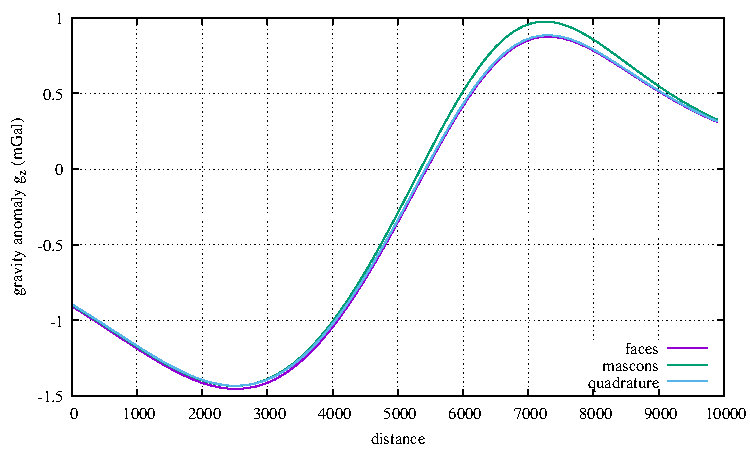
\includegraphics[width=10cm]{python_codes/fieldstone_100/results/olympus/line}
\end{center}

The measured gravity on this line for all 4 resolutions is as follows:

\begin{center}
\includegraphics[width=16cm]{python_codes/fieldstone_100/results/gravity_above_olympus_mons.pdf}\\
{\captionfont Measured gravity $|\vec{g}|$ as a function of the co-latitude.}
\end{center}

TODO: plot topography underneath. Also plot $g_r$ and not $|\vec{g}|$ ?


%----------------------------------
\subsection*{Using tetrahedra}



\begin{center}
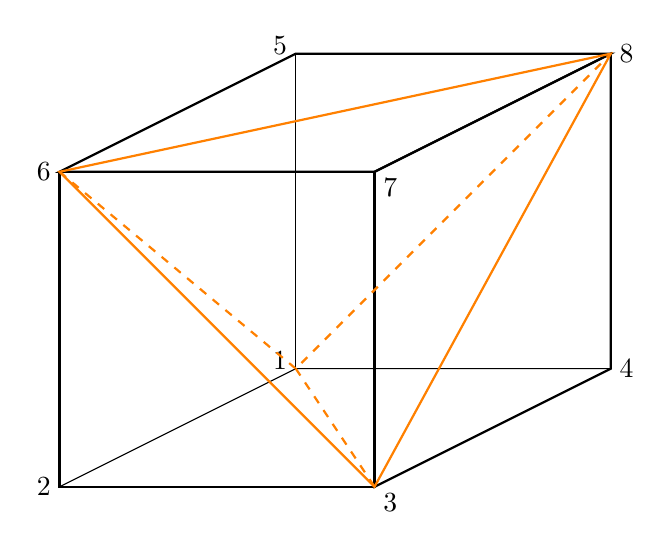
\begin{tikzpicture}
%\draw[step=0.5cm,gray,very thin] (0,0) grid (8,7); 
\draw[thick] (1,1)--(5,1)--(5,5)--(1,5)--cycle;
\draw[thick] (5,1)--(8,2.5)--(8,6.5)--(5,5)--cycle;
\draw[thick] (1,5)--(5,5)--(8,6.5)--(4,6.5)--cycle;
\draw[] (1,1)--(4,2.5)--(8,2.5);
\draw[] (4,2.5)--(4,6.5);
\node[] at (3.8,2.6) {$1$};
\node[] at (0.8,1) {$2$};
\node[] at (5.2,0.8) {$3$};
\node[] at (8.2,2.5) {$4$};
\node[] at (3.8,6.6) {$5$};
\node[] at (0.8,5) {$6$};
\node[] at (5.2,4.8) {$7$};
\node[] at (8.2,6.5) {$8$};
\draw[-,thick,orange] (1,5)--(5,1)--(8,6.5)--cycle;
\draw[thick,orange,dashed] (1,5)--(4,2.5)--(8,6.5);
\draw[thick,orange,dashed] (4,2.5)--(5,1);
\end{tikzpicture}
\end{center}

\begin{center}
\begin{tabular}{lcccc}
\hline
tetrahedron & node 1& node 2& node 3& node 4  \\
\hline
\hline
1&2&3&6&1 \\
2&4&1&8&3 \\
3&5&1&6&8 \\
4&7&8&6&3 \\
5&3&6&1&8 \\
\hline
\end{tabular}
\end{center}



